%!TEX root = vaisagh_thesis.tex
\chapter{Conclusion and Future Work}
\label{chapter:finale}

The previous chapters have introduced the IBEVAC architectures and it's constituent models. Only the IBP module has been implemented so far. The preliminary design of the remaining modules was discussed in Chapter~\ref{chapter:TheRemainingModules}. However, design work still needs to be done before the model design can be finalized. In Sect.~\ref{CFW:ModelDesign}, an expected time frame for finalizing the design details of the model is first discussed. Following this, in Sect.~\ref{CFW:Implementation}, some of the implementation details and tools used are discussed along with an estimated schedule for completion of implementation of the model. Finally, some of the work involved in validation of the model is then presented in Sect.~\ref{CFW:Validation}. However, before the future work and plan of action is discussed, Sect.~\ref{CFW:Conclusion} first summarizes and concludes the report.


\section{Summary and Conclusion}
\label{CFW:Conclusion}

In the beginning of this report, the idea of crowd egress simulation and the importance of modeling accurately the entire process of evacuation right from the pre-evacuation behavior to the time where all the evacuees have evacuated the building was introduced. Then a brief overview of the limitations of existing models. The information based approach to modeling crowd egress that is presented in this report was intorduced next.

Chapter~\ref{chapter:LiteratureReview} gave a comprehensive overview of the literature. The multidisciplinary nature of the problem was presented next; this was followed by a detailed discussion of the current state of our knowledge of human behavior process in fire evacuations. The various crowd behavior theories developed over the years was introduced and an analysis of the similarities and differences of these models was presented. This was followed by an overview of the different approaches to the problem of computationally modeling and studying a crowd evacuation. This was followed by a detailed analysis of some notable models and the strengths and weaknesses of these models.

Chapter~\ref{chapter:IBEVAC} introduced a complete information based model of an agent complete with an information based perception system, a communication engine, a memory system, a decision making engine and a navigation system.

A basic Information Based Perception~(IBP) model has already been developed and it was presented in Chapter~\ref{chapter:IBP}. The chapter also presented some simulation results that illustrated the effects of using an Information Based Perception on motion planning. In Chapter~\ref{chapter:TheRemainingModules}, the other modules in the model were presented along with some of the related work and basic details of each module.

Finally, this chapter presented a breakdown of the future work that remains along with an estimated time frame for completion of each of these tasks. These are illustrated in Fig.~\ref{fig:GanttChart}.


\section{Future Work}
\label{CFW:FutureWork}
This section discusses the work that remains to be done for the completion of this thesis. As mentioned above, this section is subdivided into three sections highlighting the work remaining in model design, implementation and validation. A Gantt chart figuratively illustrating the schedule proposed in this section is shown in Fig.~\ref{fig:GanttChart} at the end of this chapter.

\subsection{Model design}
\label{CFW:ModelDesign}

The development and implementation of any simulation model generally begins with an extensive study of the literature, followed by an identification of shortcomings in existing work and establishment of a problem to be solved. The next step is to conceptually develop a model that can in principle tackle the identified problem. This is where the process of \emph{model design} starts. In Sect.~\ref{IBEVAC:EgressProgress} of this report, the problem of accurately modeling accurately the behavior of humans in a crowd simulation was broken down into six constituent building blocks. By doing this, an overall architecture that could solve the problem at hand was developed. However, at this point, much work still remained in designing each of the remaining modules. For each module, the same process has to be repeated, i.e.\ existing work should be studied, the strengths and shortcomings of existing models, if any, should be analyzed and a design of each model along with its structure and working should be developed. During this process care should be taken to ensure that each module not only fulfills its own task but it should also work well with the remaining modules and help towards achieving the model's objective. Depending on some factors like the existing work and the modeler's experience, the design of a model can take a few days or weeks. The preliminary background studies and design work has been done for all the modules and these were discussed over the previous chapters. In the following paragraphs, the work that remains in the design of each module of the IBEVAC architecture is presented along with an estimated time to completion for those modules whose design has not been finalized.

Of the seven modules in the IBEVAC architecture, the IBP module's design has been more or less completed and it was presented in detail in Chapter~\ref{chapter:IBP} along with details of its implementation and some experiments conducted. However, as stated earlier in this report, minor work still remains in updating this perception module to obtain cue information from the environment and in detailing an approach to implementing a dynamic information limit. By a conservative estimate, 10 days would suffice to complete this work.

The proposed 4-level Navigation Module is currently being designed and implemented as an extension to the navigation system used in DEPATHSS egress simulation system. DEPATHSS will be discussed in more detail in Sect.~\ref{CFW:Implementation} along with other implementation details. For now, it is sufficient to note that the Navigation Module's design has been completed.

The background details and proposed details of the Event Knowledge Module was discussed in much detail in Sect.~\ref{CFW:EventIdentification}. The proposed model is coherent and its working and interaction with the other modules has been satisfactorily developed. While it has not been implemented and tested yet, from the perspective of model design it is reasonable to assume that the work has been fully completed.

Even though, the agent description module's working has been discussed in Sect.~\ref{CFW:ADM} details regarding its interaction with the other modules hasn't been finalized. This cannot be finalized until the other models have been finalized. However, being a small module, this work should take just about 2 days.

Section~\ref{CFW:CognitiveMap} discussed some of the most prominent work that's been done in modeling cognitive maps in robotics and simulation systems. However, a more thorough study of existing knowledge of cognitive maps and testing and validation of the proposed Environment Knowledge Module is required before the design can be finalized. The designing of the model should involve about 25 days work.

The Communication Module~(Sect.~\ref{CFW:CommunicationModule}) is in a similar state to the Environment Knowledge Module, not least because its working is highly dependent on the latter's structure and working. A similar estimate of 15 days work to be done concurrently with the environment knowledge module is made.

The basic details of the working of the Planning Module was presented in Sect.~\ref{CFW:Planner}. While this is coherent and its interaction with the other modules are relatively clear, the actual strategies to be implemented and the constituent tasks have not been developed. The relevant literature about normal tasks that are carried out by individuations has been analyzed and presented in Sect.~\ref{LiteratureReview:CurrentUnderstanding}. However, some tasks are highly context dependent and cannot be finalized until the exact details of the scenario are finalized. This work can take up to 25 days.

% Requires the booktabs if the memoir class is not being used
\begin{table}[tbp]
\centering
\topcaption{Time-frame for tasks in Model Design} % requires the topcapt package
\begin{tabular}{p{2.5in}   p{1.25in}   p{1.25in}} % Column formatting, @{} suppresses leading/trailing space
\hline\hline %inserts double horizontal lines
Task & Percentage Work Completed & Estimated Time to Completion \\
\hline
Overall Architecture  & 100\% & - \\[3pt]
IBP Module  & 90\% & 10 days \\[3pt]
Navigation Module  & 100\% & - \\[3pt]
Event Knowledge Module & 100\% & - \\[3pt]
Environment Knowledge Module & 60\% & 25 days \\[3pt]
Agent Description Module  & 70\% & 2 days \\[3pt]
Communication Module  & 60\% & 15 days \\[3pt]
Planning Module  & 70\% & 25 days \\[3pt]
\hline
Total  & 93\% & 51 days \\[3pt]
\hline
\end{tabular}
\label{tab:ModelDesign}
\end{table}


\subsection{Implementation and simulation}
\label{CFW:Implementation}

The \emph{implementation} of a model refers to the process of converting the conceptual design into code, i.e.\ a computational model. The section presents some of the details of the implementation like the tools used and the existing work on which the model is built. Section~\ref{CFW:TimeFrame} then presents an estimated time-frame for completion of different implementation related tasks.


\subsubsection{The MASON framework}
\label{CFW:MASON}
The IBEVAC model is implemented in Java using the MASON framework~\cite{Luke:2005wc}. MASON consists of a discrete event simulation core and visualization library that can be used for agent based simulations with a large number of agents. The framework provides features to allow modelers to run multiple replications and create checkpoints from which simulations can be restarted easily. The ease of implementation of inspectors to study particular agents or other aspects of the model and integration with java media framework library (for videos and snapshots), jGraph and java3D make MASON especially appealing for the purpose of this simulation. The framework internally adopts the model-view-controller pattern and completely decouples the view from the controller and the model and makes it easy for a modeler to adopt the same approach. This is critical for studying simulations because a visualization need only be used when particular parts of the simulation need to be observed and analyzed and at all other times more simulations can be run without the additional computational burden of visualization.



\subsubsection{DEPATHSS}
\label{CFW:Depathss}

DEPATHSS is a simulation system for symbiotic simulations of evacuation scenarios (Screenshot in Fig.~\ref{fig:DEPATHSSScreenShot}). It is not directly related to the IBEVAC model. However, the Java based implementation of the simulation system provided a good starting point for implementation of the IBEVAC model and helps remove a lot of programming work that might have been required if the model had to be implemented from scratch.

A Finite Difference Model based implementation of fire propagation used in DEPATHSS is adapted to the MASON framework to simulate fire and smoke propagation in IBEVAC. The smoke will be given a higher diffusion rate so that it spreads at a faster rate.

\begin{figure}[!tb]
\centering
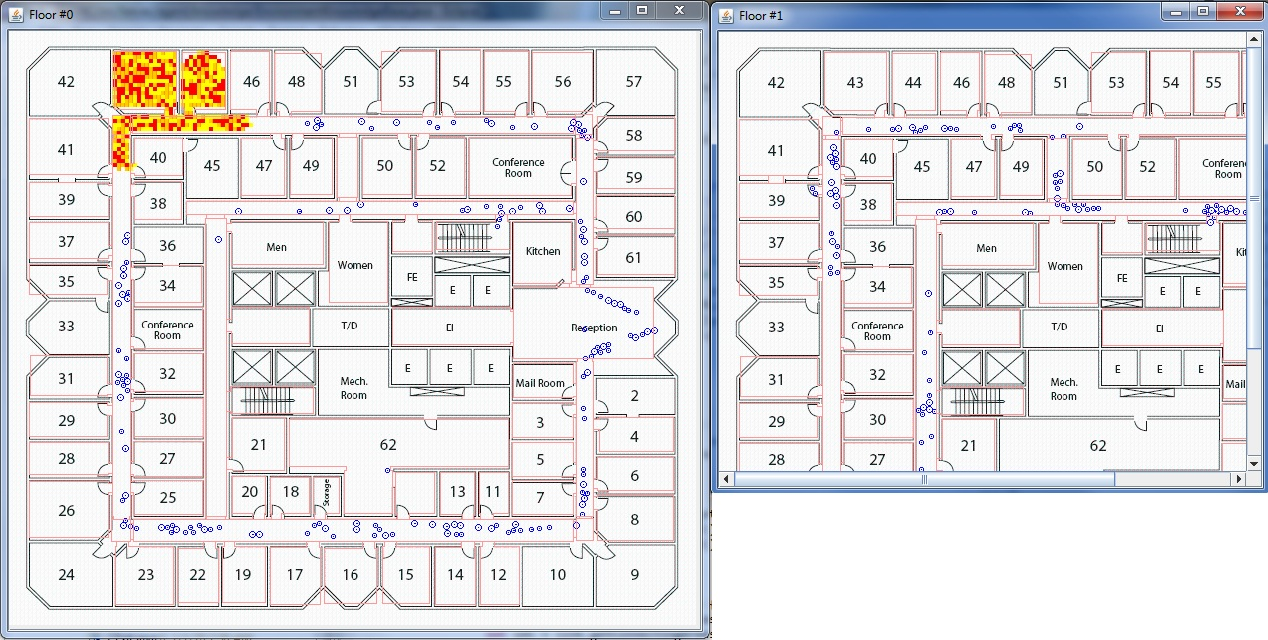
\includegraphics[width=\textwidth]{HiekoSimulationMultiFloor}
\caption[DEPATHSS Screenshot]{This figure shows a screenshot of the evacuation simulation using DEPATHSS of a 2-floor office building with fire propogation modelled (The red, yellow and orange color at the top left of the screen on the first floor). Agents are in blue.}
\label{fig:DEPATHSSScreenShot}
\end{figure}

Another very useful feature of the DEPATHSS system is the ability to create and store layouts of buildings in a generic XML format that can be easily imported into the model. This will be invaluable during experimentation and validation.

As mentioned earlier, the DEPATHSS system's navigation system is being extended to use the 4-level navigation architecture mentioned in this paper. This navigation system can also be integrated into the IBEVAC architecture without much difficulty.

Like the navigation system DEPATHSS is also currently being extended with simple personal cognitive maps for agents and knowledge transfer between agents. This can initially be used in IBEVAC while developing the other modules. Once the other modules have been developed the Communication and Environment Knowledge Modules can be modeled as required by replacing the existing system.

All this implies that, most of the lower level tasks like the framework, basic goal directed navigation and fire and smoke simulation have been completed and tested and most of the work remains only in implementing a higher level behavioral model which is the key contribution of this thesis. An estimate of the time frame required for different aspects of this implementation is considered next.

\subsubsection{Time frame for model implementation}
\label{CFW:TimeFrame}

% Requires the booktabs if the memoir class is not being used
\begin{table}[tbp]
\centering
\topcaption{Time frame for tasks in Model Implementation} % requires the topcapt package
\begin{tabular}{p{2.5in}   p{1.25in}   p{1.25in}} % Column formatting, @{} suppresses leading/trailing space
\hline\hline %inserts double horizontal lines
Task & Estimated Time to Completion \\
\hline
Preliminary Model  & 16 days \\[3pt]
IBP Module Integration  & 15 days \\[3pt]
Event Knowledge Module    & 35 days \\[3pt]
Planner   				& 45 days \\[3pt]
Agent Description Module  & 5 days \\[3pt]
Environment Knowledge     & 20 days \\[3pt]
Communication Module 	& 20 days \\[3pt]
\hline
Total & 12 weeks \\[3pt]
\bottomrule
\end{tabular}
\label{tab:Implementation}
\end{table}

Even though, the aforementioned DEPATHSS system has been developed in Java it is not integrated with the MASON framework whose features and strengths mentioned in Sect.~\ref{CFW:MASON} would be extremely useful. Besides this, some work has to be done in integrating the features of DEPATHSS into an IBEVAC like architecture. Thus the first objective in implementing the model would be to create a simple simulation system where a group of agents simply move towards the exit of a building. This preliminary system will not be implementing any higher level behavior. This process can take up to 16 days.

The next step in implementation would involve integrating the Information Based Perception system into this simulation system. While the IBP module has been implemented and tested, this implementation and testing were done in a different much simpler framework. However, the implementation was in Java and using Mason, so 15 days would be sufficient to complete the implementation of the IBP module.


As mentioned in the previous section, there already exists a simple version of the Environment Knowledge Module and the Communication Module. Thus the development of the more complicated IBEVAC version of these modules with notions of trust and forgetfulness can be put on hold till after the Planning Module and Event Knowledge Module have been developed. The Planning Module will have to be initially implemented with some simple strategies because it is essential to the working of the Event Knowledge Module. In fact, both these modules will have to be developed in parallel because they are highly interconnected in their working. This process will also involve upgrading the IBP module to perceive cues from the environment. This would be the most substantial work involved in the implementation of the model. We estimate that this can take about 50 days.

Next the Agent Description Module can be developed. While this module itself is not that complicated; implementing this module will result in changes in the Event Knowledge Module and the strategies in the Planner. This will take about a week to implement.

Finally, the Communication and Environment Knowledge Module will have to be modified and changed to work as specified in the IBEVAC model. This will take about 20 days to implement.

\subsection{Validation}
\label{CFW:Validation}

Validation for crowd simulation is a very difficult problem for which there isn't any accepted solution. Especially in the present case of a system that models and simulates a fire evacuation, it is ethically and practically impossible to actually start a fire and observe the evacuees.

In general, macroscopic models like the lattice gas models validate their model by simulating the evacuation from a room and constructing a graph of the rate of evacuation against time~\cite{Nagai:2004kl}. This method might ensure accurate macro level behavior but gives no guarantee of the micro level accuracy or behavior of the model. This is of little use to civil defense or fire authorities trying to figure out a way to limit the damage caused by fires.

Pelechano~\cite{Pelechano:2008uo} and the Gamma group at University of North Carolina~\cite{Snape:2009er,Guy:2010ko,vandenBerg:2008cq} use the presence or absence of certain characteristics of motion like \emph{reciprocal dances}~\cite{Snape:2009er,vandenBerg:2008cq} and continuity of the movement~\cite{Pelechano:2008uo} to measure the realism of the movement. A somewhat related method is one that uses visual validation. In this approach, videos or actual crowds are observed and certain patterns are observed; The model is validated by checking its ability to produce similar patterns and behavior.

Comparing against videos of crowds moving is a reliable method for validation. But according to Banerjee et al.~\cite{Banerjee:2011uz}, what is missing is a clear and reliable method for ensuring that the validation is accurate. To counter this problem, they have suggested a system for quantitative validating agent based crowd simulation systems. They use a novel, automated method for comparing the results~(the movements) produced by the simulation against videos of crowds evacuating from a stadium that are available from CCTVs. They call this method quantitative validation. The area in the simulation is first divided into regions. The movement produced in each of these regions is compared against the movement in the video. A similar method is also used in other studies~\cite{Lerner:2009wj,Lerner:2010cu}. They have verified the working of this automated method by validating a model of evacuation from a stadium. This method of quantitative validation is unlikely to be useful in a fire evacuation simulation because it is difficult, if not impossible, to get videos of crowds taking part in an actual fire evacuation.

The best records of peoples actions during fires and evacuations is available through interviews of the evacuees. Various studies~\cite{Torres:2010tj,Cocking:2007wp,Kobes:2009jx,Purser:2001ts} give a very accurate account of people's behaviors during fires. Models of fire evacuation can start of by trying to produce the sorts of actions that were revealed in these interviews. This brings us to the concept of micro validation. In this method, rather than trying to produce the complete, detailed real life situation ``as is'' in a computer simulation, we try to produce and verify certain actions and behaviors that were characteristic of the evacuation. Realistically speaking, this is all that can be expected from the system, because it is impossible to predict the movement of every person in an evacuation without at least having a complete and comprehensive personal history of the person. This is not \emph{that} severe a limitation because it still gives a fairly good idea of the crowd's reaction.

Data plays an important part in validating these multi agent systems. The more data, the better a system can be validated. But as the scale of the system and its complexity of the system increases, interviews and surveys become progressively less useful. Another method for validating agent based systems, especially human behavior is by using the power of human computation~\cite{VonAhn:2007wi}.

In~\cite{Pengfei:2011us}, we suggested a methodology that used key ideas from human computation as a means of collecting large amounts of contextual behavioral data. They key principle of this approach is to design games such that they act as a means of framing behavioral questions to try and capture people's natural and instinctive decisions. This method has the key advantage of being able to generate large sets of data from a large sample set. The approach also offers the advantages outlined by Sterman~\cite{Sterman:1987vk}, in that using carefully designed scenarios and games provides a more contextual and interactive form for phrasing a question.

In the context of validation, it might be interesting and relevant to mention the work we are currently doing in comparing the results produced by social forces~\cite{Helbing:2000ef} and RVO2~\cite{Guy:2010ko} against a simple lattice gas model~\cite{Nagai:2004kl} when simulating simple situation like exit from a room or merging of two paths.

A combination of the different approaches for validation that are available will be used to validate the IBEVAC model. Validation is a continuous process that begins right from the point of development of the model. The validation period consists of planning and running experiments on the simulation, gathering data and debugging the model.

\subsubsection{Validation}
\label{CFW:ValidationTimeFrame}

% Requires the booktabs if the memoir class is not being used
\begin{table}[tbp]
\centering
\topcaption{Breakdown of tasks in Validation} % requires the topcapt package
\begin{tabular}{p{2.5in}   p{1.25in}   p{1.25in}} % Column formatting, @{} suppresses leading/trailing space
\hline\hline %inserts double horizontal lines
Task & Estimated Time to Completion \\
\hline
Phase 1: Literature Review & 30 days \\[3pt]
Phase 2: Planning & 90 days \\[3pt]
Phase 3: Experimentation & 100 days \\[3pt]
Phase 4: Analysis & 100 days \\[3pt]
\hline
Total & 17 weeks \\[3pt]
\bottomrule
\end{tabular}
\label{tab:Validation}
\end{table}

To determine an estimated time frame for the validation process, it is helpful to divide this process of validation into four phases.

Firstly, existing work on validation will have to be studied in detail to understand the pros and cons of different approaches to validation. While some of the work has been done in this regard, three to four weeks will have to be spent in consolidating this knowledge of existing validation methodologies.

Next, based on this literature and the module being validated, different experiments and will have to be designed for verifying and validating the working and effect of each module on the agent's behavior. These experiments can be in the form of scenarios to be run on the simulation or actual real world experiments or experiments conducted on the aforementioned use of human computation~\cite{Pengfei:2011us}. This process will take a considerable amount of planning. However, the major portion of this work will be done alongside the third phase of the validation process which involves conducting these planned experiments and gathering data.  However, the process of running simulation experiments and collecting data can be automated to an extent through scripts. This enables more work on phase 2 and 4 to be done while the data is being generated. A period of 115 days is allotted for completing phases 2 and 3 of validation.

The fourth and final phase of validation involves aggregating the collected data and analyzing it. At this point changes might have to be made in the model and further experiments might have to be planned and implemented. A period of 100 days is alloted to this phase. It is important to note the unlike the development and implementation tasks, validation tasks are generally more open ended~(except for phase 1). Hence work on validation is likely to continue till very near the date of thesis submission.


\begin{sidewaysfigure}[!tb]
\centering
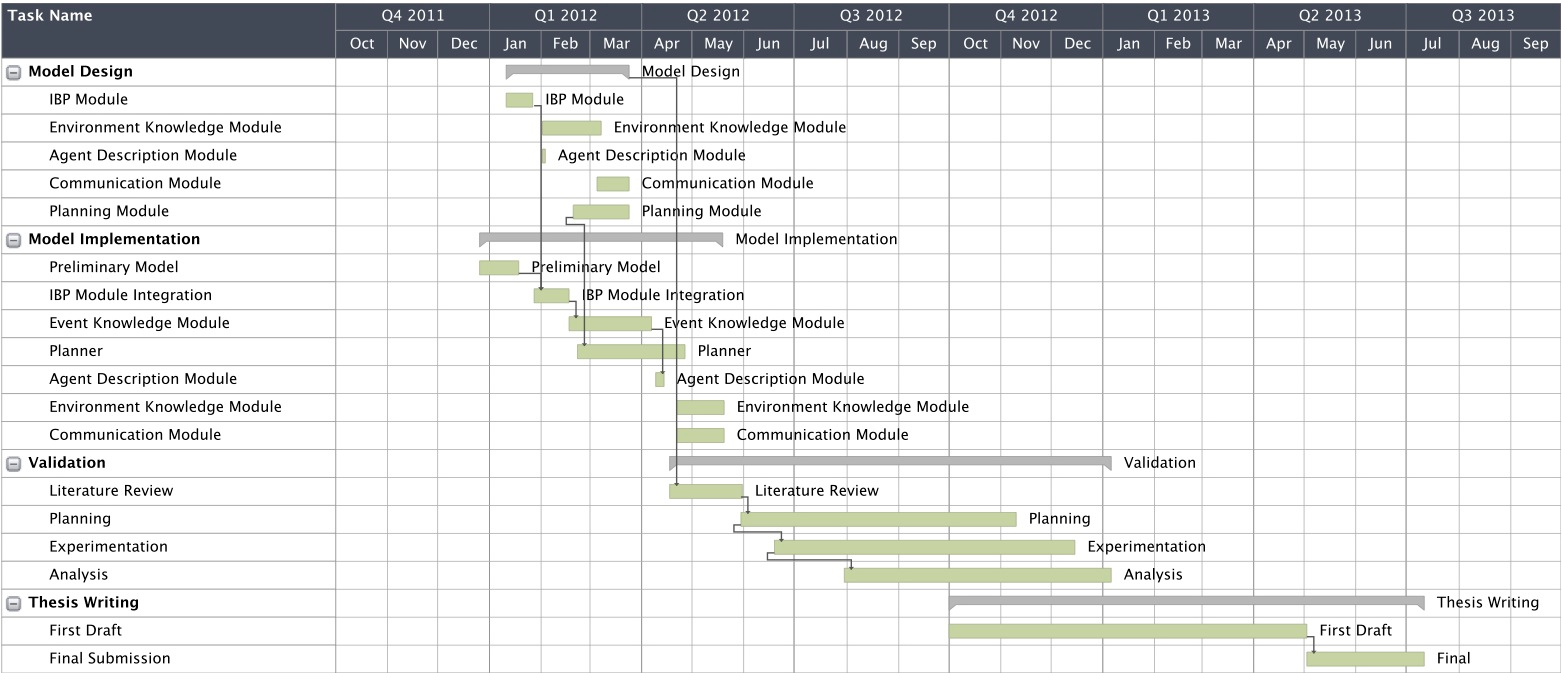
\includegraphics[width=\textheight]{GanttChart}
\caption[Planned Schedule]{Gantt Chart showing the plan of action for the present thesis. The chart excludes weekends, public holidays and 21 days a year from the calender to account for allowed leave.}
\label{fig:GanttChart}
\end{sidewaysfigure}

